\chapter{Ingénierie des exigences}
\section{Approche Top-Down}
\label{sec:top-down}

Pour notre approche Top-Down, nous sommes revenus à la demande initiale du projet : remplacer la souris d'un ordinateur par le mouvement oculaire de l'utilisateur. La fonction principale du système est donc apparue clairement : permettre à l'utilisateur d'interagir avec une interface via ses yeux. 

\begin{figure}[h]
  \centering
  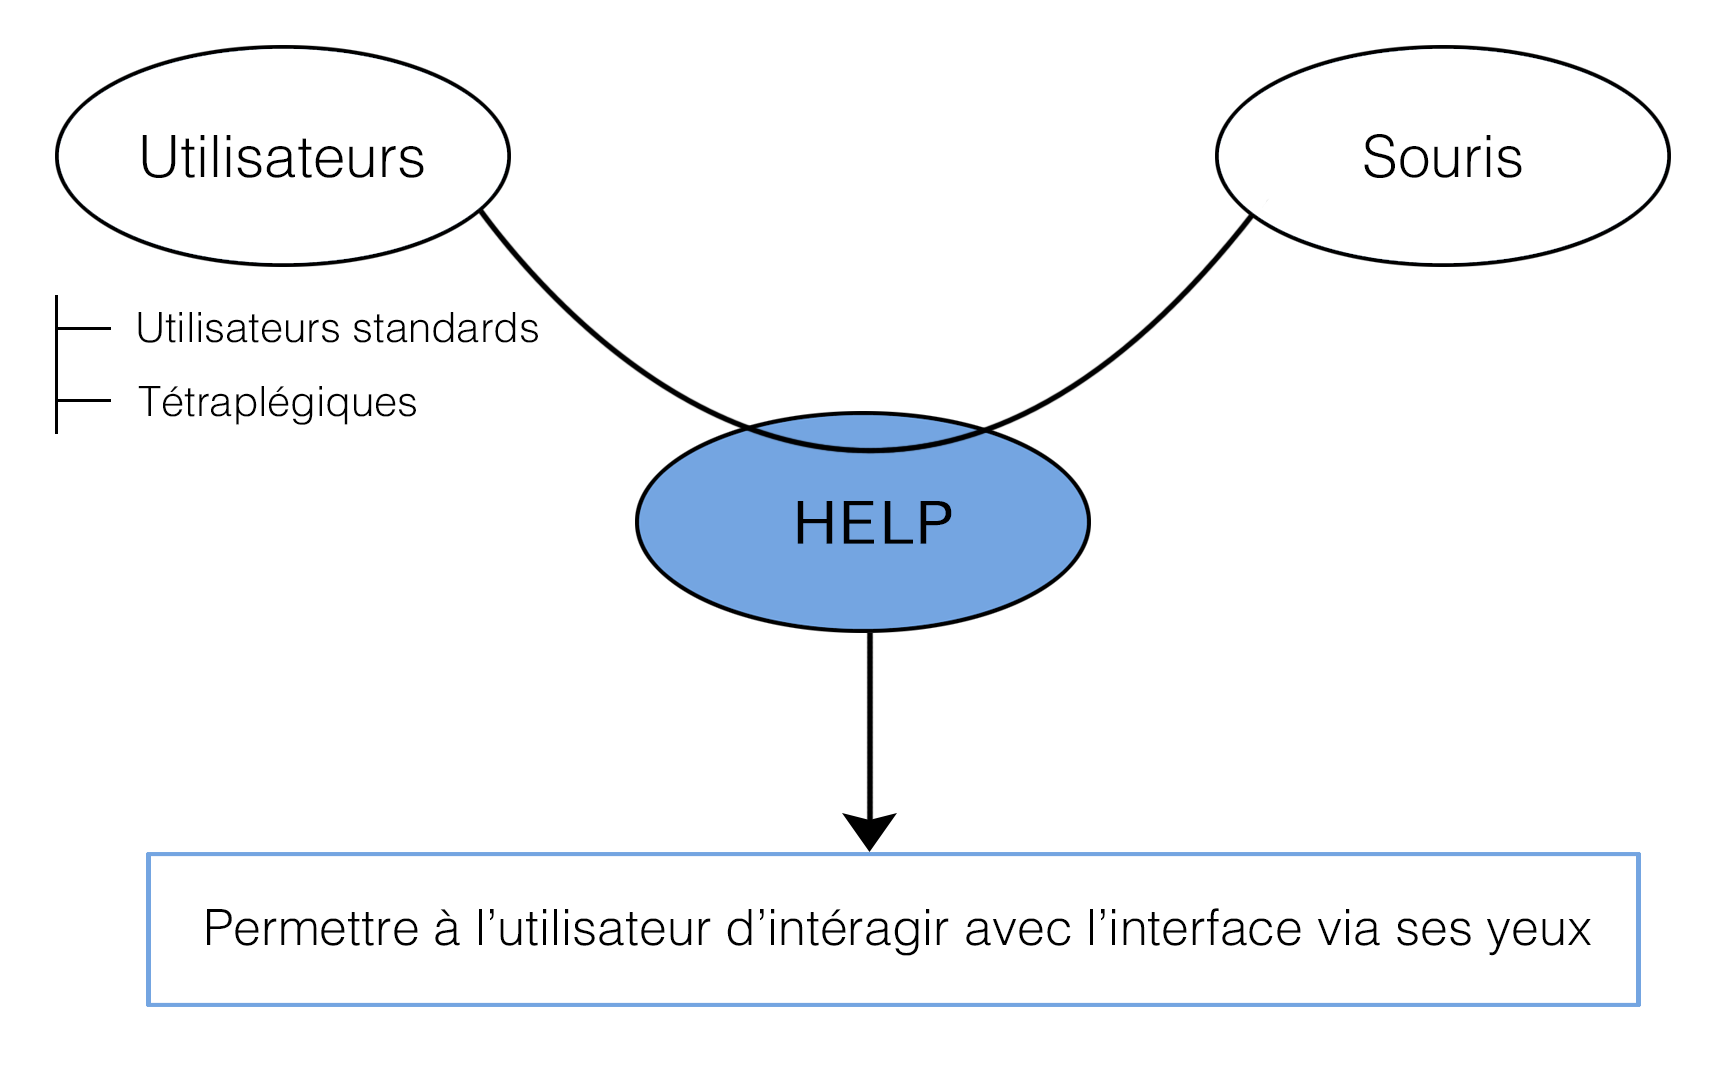
\includegraphics[scale=1]{BeteACornes}
  \caption{Bête à cornes}
  \label{fig:bac}
\end{figure}

\begin{figure}[H]
  \centering
  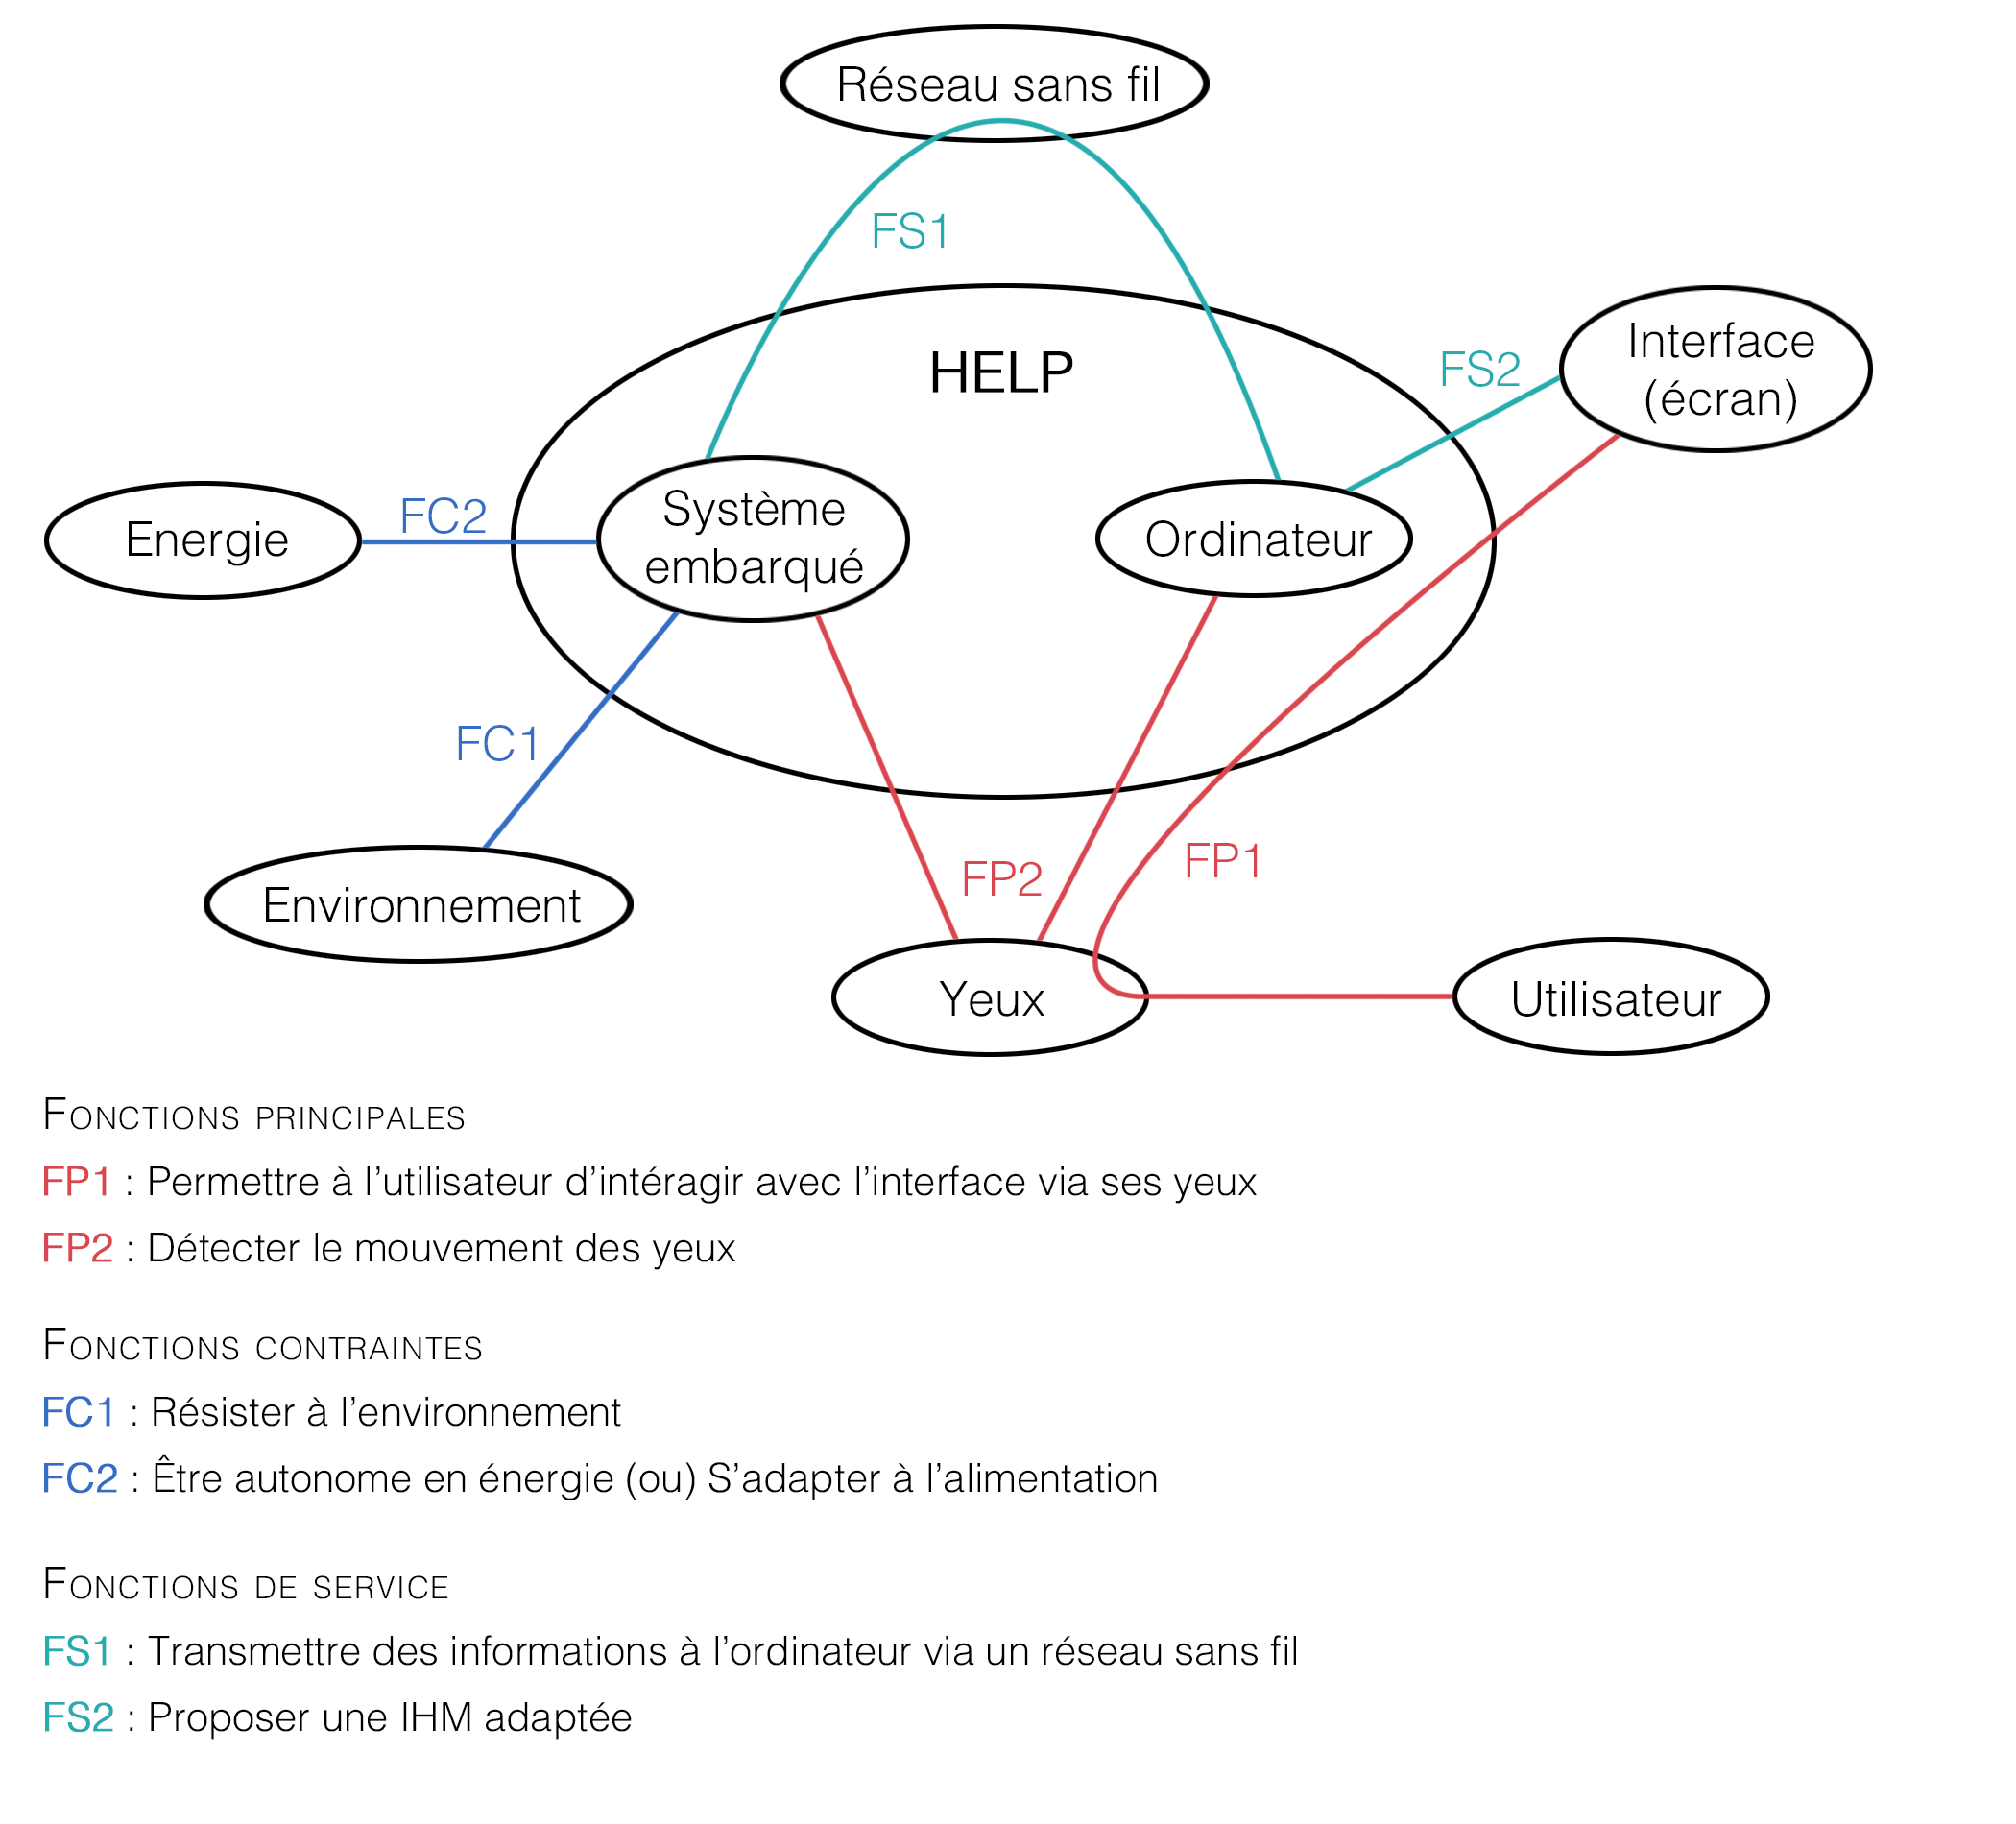
\includegraphics[scale=0.9]{Pieuvre}
  \caption{Diagramme pieuvre}
  \label{fig:pieuvre}
\end{figure}

\section{Approche Bottom-Up}

Nous avons défini les différentes exigences auxquelles le système devra répondre, indépendamment de nos choix de réalisation technique. Nous les avons alors rassemblées par groupement logique, ce qui nous permettra de définir nos fonctions principales. 

\begin{figure}[H]
  \centering
  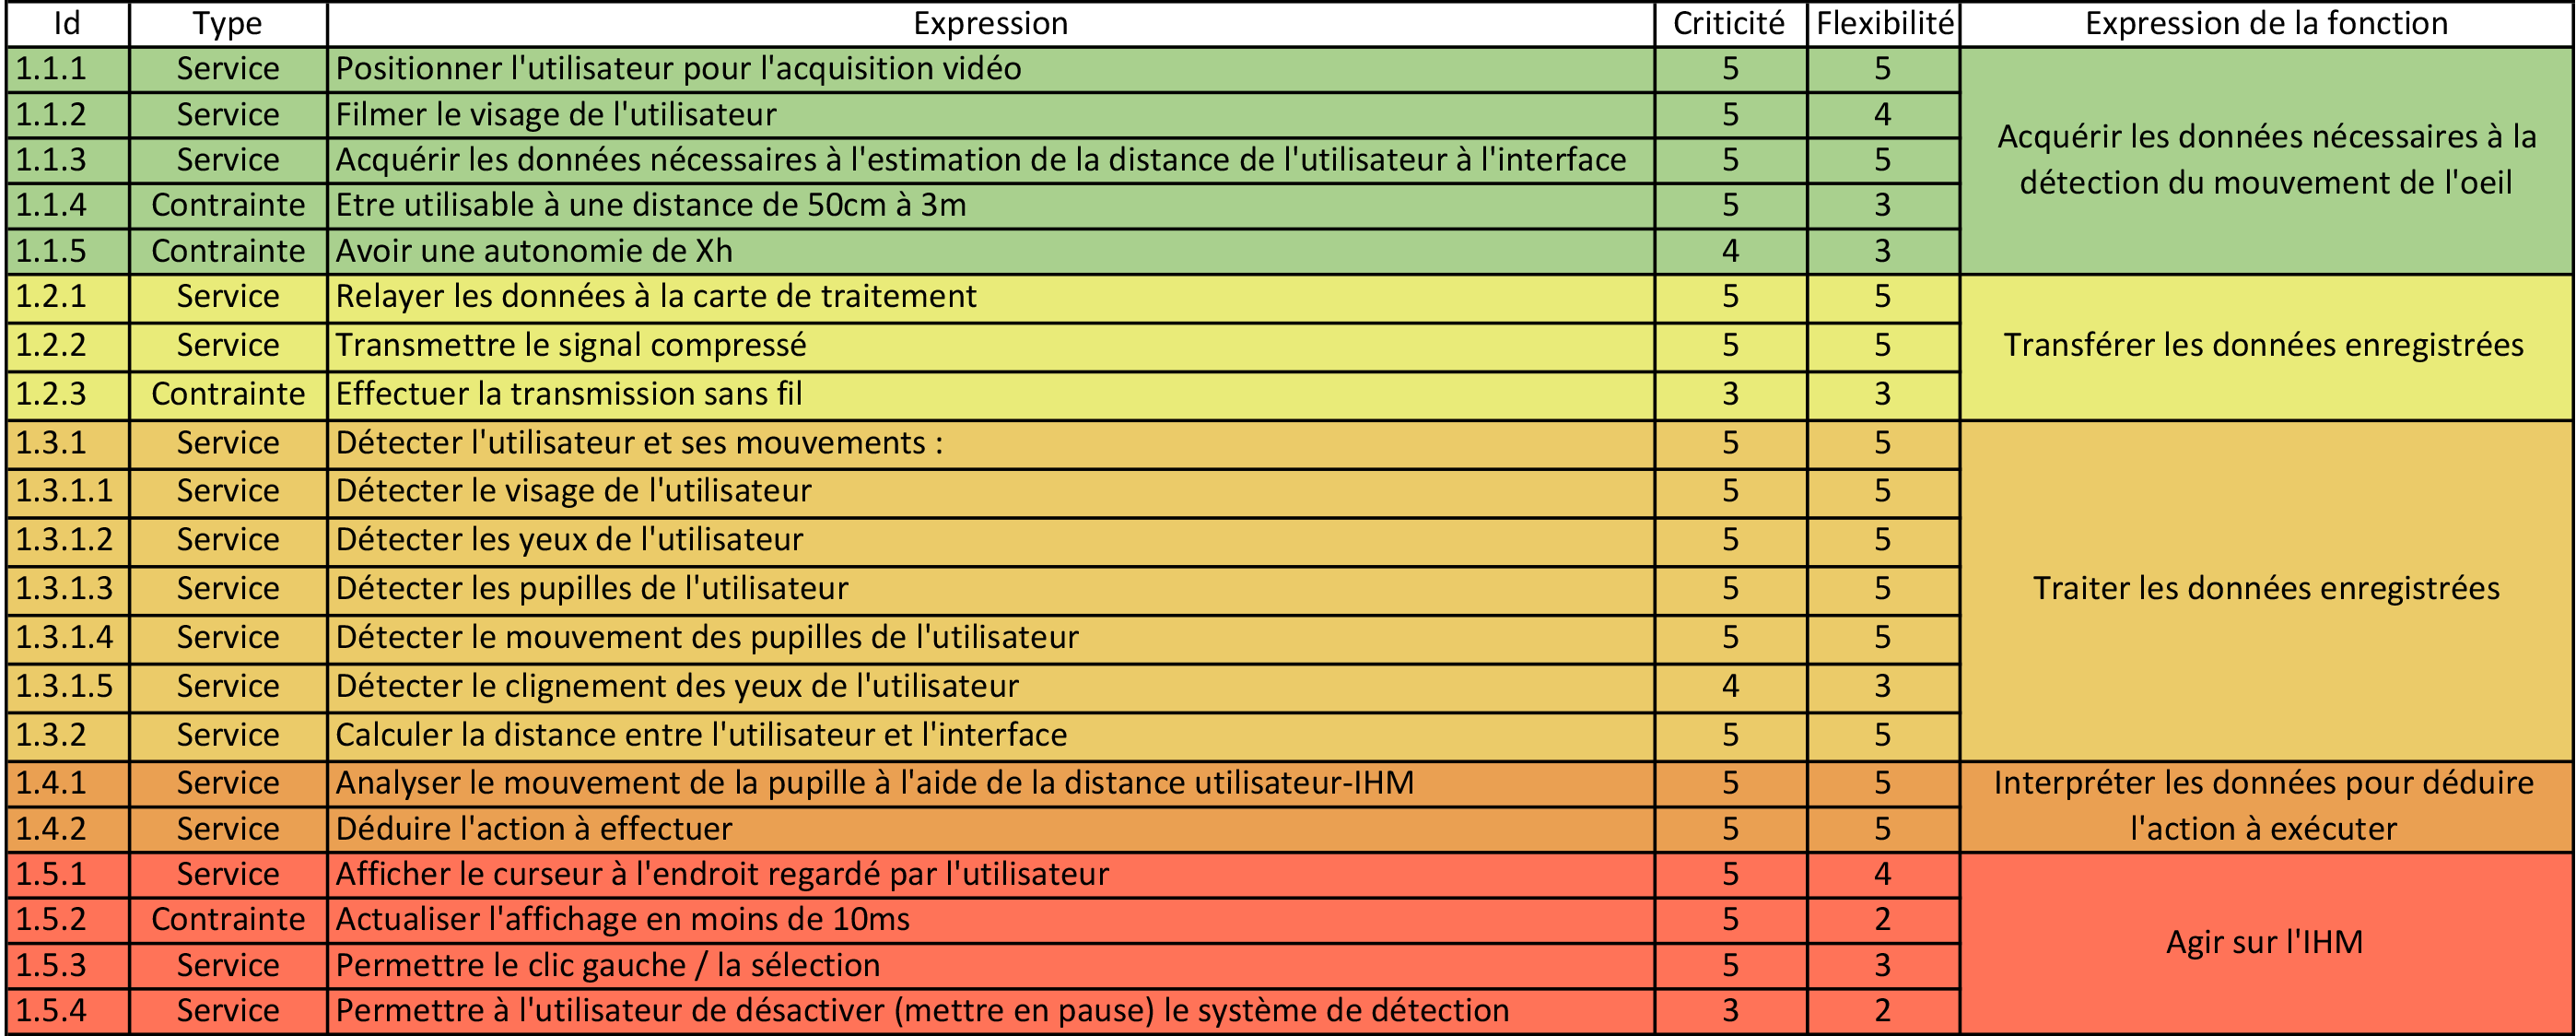
\includegraphics[width=\textwidth]{CahierdesExigences}
  \caption{Cahier des exigences}
  \label{fig:exigences}
\end{figure}

\section{Fonctions principales du système}

Dans le cadre de ce projet, nous cherchons donc à remplacer la souris d'un ordinateur par un système qui suit le mouvement des yeux de l'utilisateur. Pour ce faire, nous avons mis en évidence des groupements logiques d'exigence. Tout d'abord, le système doit acquérir les données nécessaires à la détection du mouvement de l'œil. Ces données devront alors être transférées, puis traitées par l'ordinateur. Ce dernier doit alors interpréter ces données pour en déduire l'action à exécuter. De ces nouvelles informations, l'ordinateur doit pouvoir effectuer l'action que l'utilisateur veut effectuer sur l'IHM, la mettre en place, et montrer que ces modifications ont été exécutées. 

\begin{itemize}[label=\textbullet,font=\color{black}]
\item FP1 : Acquérir les données nécessaire à la détection du mouvement de l'œil 
\item FP2 : Transférer les données enregistrées 
\item FP3 : Traiter les données enregistrées 
\item FP4 : Interpréter les données pour déduire l'action à exécuter 
\item FP5 : Agir sur l'IHM 
\end{itemize}

\chapter{Spécification fonctionnelle  3 axes}

\section{Raffinement FAST}

Le cahier des exigences précédant nous a permis de définir les fonctions principales du système. Nous avons alors cherché à les raffiner par la méthode FAST pour obtenir des fonctions plus précises auxquelles nous pourront apporter des solutions techniques propres à chacune. Nous pouvons ainsi entrevoir l'architecture fonctionnelle.

\begin{figure}[H]
  \centering
  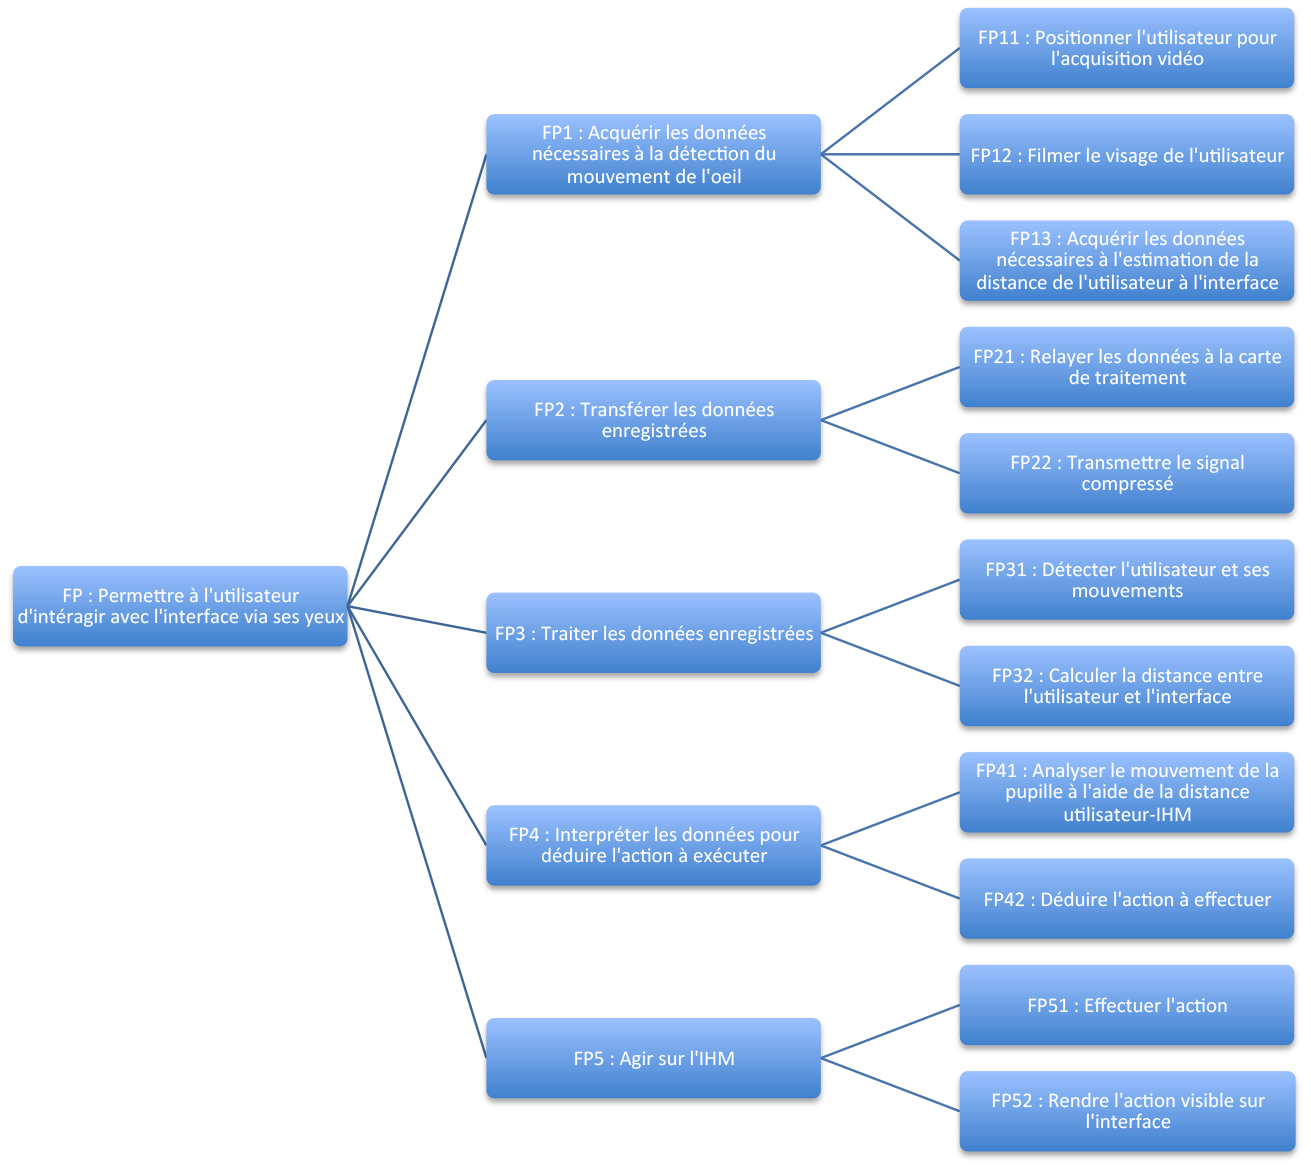
\includegraphics[scale=1.2]{FAST}
  \caption{FAST raffiné}
  \label{fig:FAST}
\end{figure}

\section{Spécification des données}
\section{Spécification des comportements}


\chapter{Architecture fonctionnelle}


